\section*{Введение}
\addcontentsline{toc}{section}{Введение}

\textbf{Полярные сияния} (aurora borealis на севере и aurora australis на юге) --- одни из самых красивых природных явлений. Их наблюдали тысячи лет, но крепко поняли только во второй половине XX века с развитием космической физики. Сегодня известно, что сияния появляются, когда заряженные частицы от Солнца взаимодействуют с магнитным полем и атмосферой Земли~\cite{kivelson1995}.

\begin{figure}[H]
    \centering
    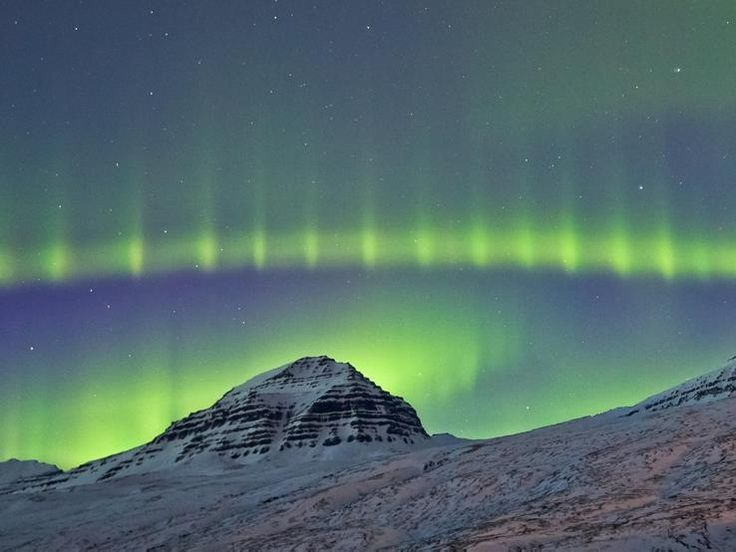
\includegraphics[width=0.8\textwidth]{images/aurora1.jpg}
    \caption{Полярное сияние (Aurora Borealis)}
    \label{fig:aurora1}
\end{figure}

Тема важна не только из-за интереса к процессам между Солнцем и Землей, но и из-за практики. Авроральная активность --- заметный пример космической погоды. Сильные магнитные бури с яркими сияниями могут сбивать спутники, влиять на линии электропередач, трубопроводы в высоких широтах и мешать радиосвязи и GPS. Поэтому понимание механизмов сияний полезно и в науке, и на практике.

\textbf{Цель работы} --- собрать и систематизировать физику возникновения полярных сияний, описать их виды и факторы, которые влияют на них.

Для достижения цели нужно:
\begin{enumerate}
    \item Проследить, как менялись представления о полярных сияниях с древности до наших дней.
    \item Рассмотреть главные физические процессы: пересоединение магнитных линий, ускорение частиц и возбуждение газов атмосферы.
    \item Классифицировать виды сияний и связать их внешний вид с условиями их появления.
    \item На основе литературы оценить, какие направления в исследованиях перспективны, а какие нет.
\end{enumerate}

Объект исследования --- полярные сияния как природное явление. Предмет --- физика их возникновения, виды и влияющие факторы.